O GuppyLM é um modelo de linguagem deliberadamente minúsculo, de código aberto e orientado
a caracteres, tematizado como um peixe. Ele foi construído para o ensino, sendo uma
implementação de referência completa e legível de um pequeno \textit{transformer} ajustado
por instruções, e é um bom banco de provas de mecanismos precisamente porque é pequeno o
bastante para ser inteiramente controlável e inspecionável enquanto ainda é um
\textit{transformer} ajustado por instruções de verdade. Sua arquitetura e seus dados de
treinamento estão resumidos na Tabela~\ref{tab:guppylm_properties}.

\begin{table}[htbp]
\centering
\caption{Arquitetura e dados de treinamento do GuppyLM.}
\label{tab:guppylm_properties}
\begin{tabular}{l l}
\toprule
\textbf{Propriedade} & \textbf{Valor} \\
\midrule
Parâmetros &  $\approx 8{,}73$M \\
Blocos \textit{transformer} & 6 \\
Dimensão oculta $k$ & 384 \\
Capacidade de vocabulário & 4096 \\
Dados de treinamento & \href{https://huggingface.co/datasets/arman-bd/guppylm-60k-generic}{$\approx 60$ mil linhas em 60 categorias} \\
\bottomrule
\end{tabular}
\end{table}

Cada bloco emite um tensor de fluxo residual (\textit{residual stream}) de formato
$[B, T, 384]$, o que coincide com o método de Beaglehole et al. para a leitura e a escrita
no modelo. O modelo é treinado sobre 60 categorias conversacionais moldadas por
\textit{templates}, tais como comida, clima, saudações e humores, e essas categorias são
os únicos conceitos que se pode plausivelmente esperar que o GuppyLM represente, dado que
elas constituem a totalidade de sua distribuição de treinamento, razão pela qual
restringimos este trabalho a elas. Note que se o modelo carrega também estrutura para
além dessas categorias não é algo que tenhamos testado, e não é algo que uma
\textit{probe} restrita a esses rótulos pudesse enxergar.

Uma consequência conveniente da pequena escala do GuppyLM é que as normas de suas
ativações por bloco são pequenas e podem simplesmente ser medidas. A mediana de
$\|a_\ell\|_2$ sobre as ativações de treinamento armazenadas percorre
$11{,}9,\ 22{,}8,\ 27{,}6,\ 30{,}7,\ 30{,}9,\ 29{,}7$ do bloco 0 ao bloco 5, uma subida de
aproximadamente $2{,}6$ vezes que atinge seu pico no bloco 4, conforme mostra a
Figura~\ref{fig:activation_norms}. Por consequência, uma perturbação absoluta fixa é um
empurrãozinho no bloco 5 e uma bola de demolição no bloco 0, o que é exatamente a razão
pela qual os coeficientes absolutos de \textit{steering} de Beaglehole et al. não podem ser
copiados para cá.

\begin{figure}[htbp]
    \centering
    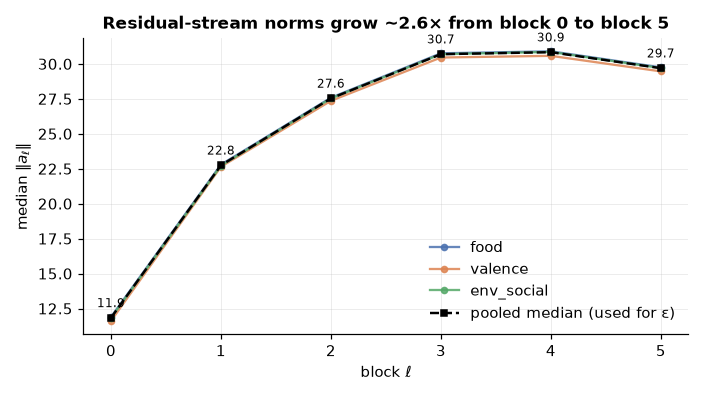
\includegraphics[width=0.75\textwidth]{imgs/01_activation_norms.png}
    \caption{Os três conceitos concordam quase exatamente, e a mediana (tracejada) é uma escala segura para a normalização.}
    \label{fig:activation_norms}
\end{figure}

É possível perceber na figura que os três conceitos concordam quase exatamente quanto ao
perfil de normas por bloco, o que significa que a mediana é uma escala comum segura para a
normalização, e é essa mediana que define o coeficiente relativo $r$ utilizado ao longo de
todos os experimentos de \textit{steering} adiante.

